\begin{figure}[t]
\centering
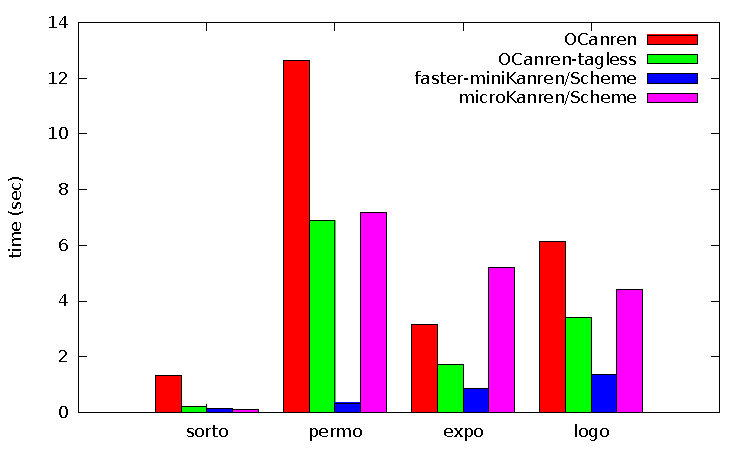
\includegraphics{graph1.pdf}
\caption{The First Set of Benchmarks}
\label{eval:first}
\end{figure}
\begin{figure}[t]
\centering
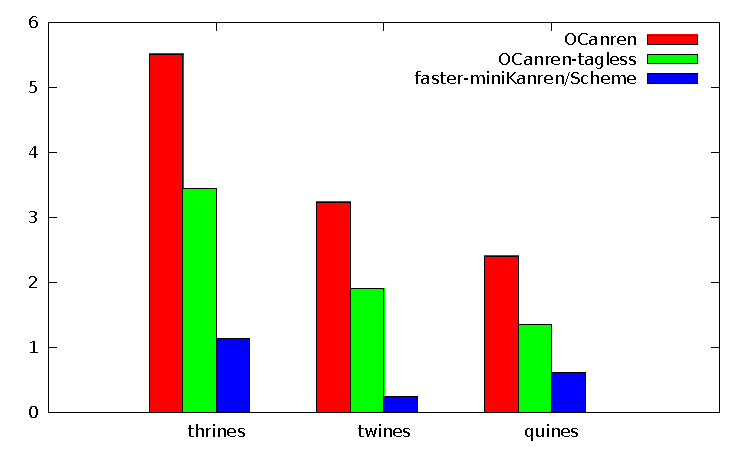
\includegraphics{graph2.pdf}
\caption{The Second Set of Benchmarks}
\label{eval:second}
\end{figure}

\section{Performance Evaluation}
\label{sec:evaluation}

One of our initial goals was to evaluate, what performance impact would choosing
OCaml as a host language make. In addition we spent some efforts in order to implement \miniKanren in
efficient, tagless manner, and, of course, the outcome of this decision also has to be measured. 
Since our library generally follows $\mu$Kanren\footnote{https://github.com/jasonhemann/microKanren}, we've chosen it as a reference implementation.
In addition, we took \texttt{faster-miniKanren}\footnote{https://github.com/webyrd/faster-miniKanren}~--- more elaborated 
implementation with a little different search~--- since it implements disequality constraints. 

For the set of benchmarks we took the following problems:

\begin{itemize}
\item \textbf{sorto, permo}~--- sorting and permutation for lists of Peano numbers (shown as example in Section~\ref{sec:examples}).
The concrete tests sort and take all permutations of list \lstinline{[4; 3; 2; 1]}.
\item \textbf{expo, logo}~--- exponentation and logarithm for integers in binary form. The concrete tests relationally compute
$3^5$ (which in 243) and $log_3 243$ (which is, conversely, 5).
\item \textbf{quines, twines, trines}~--- self/co-evaluating program construction problems from~\cite{Untagged}. The
concrete tests take first 100, 15 and 3 answers for these problems respectively.
\end{itemize}

Since the last bundle of benchmarks uses disequality constraints (and, hence, $\mu$Kanren is ruled out) we
split all benchmarks into two sets. 

The evaluation was performed on a desktop computer with Intel Core i7-4790K CPU @ 4.00GHz processor and 32GB of memory.
For OCanren \mbox{\texttt{ocaml-4.04.0+frame_pointer+flambda}} was used, for other implementations~--- Chez~Scheme~9.4.1. 
All benchmarks were run in natively compiled mode ten times, then average user time was taken. The results of evaluation
are shown on Figures~\ref{eval:first} and~\ref{eval:second}. The whole evaluation repository with scripts and detailed
description is accessible from \lstinline{gitHub}\footnote{https://github.com/Kakadu/ocanren-perf}.

The first conclusion, which is rather easy to derive from the results, is that ``taglessless'' indeed matters. Our initial
implementation did not show essential speedup in comparison with $\mu$Kanren (and was even \emph{slower} on the logarithm 
and permutations benchmarks). The situation was improved drastically, however, when we switched to a tagless version.

Yet, in comparison with \texttt{faster-miniKanren} our implementation is still lagging behind. We did not discover the exact
reasons yet, but presume, that the difference in search plays an important role here. 
We save this problem for future research.
